\subsubsection{Degree 2} $P_2(x)=a_0x^0+a_1x^1+a_2x^2=ax^2 +bx +c$, $a\ne 0$. This is known as a quadratic polynomial. There are three common ways to solve the quadratic equation $ax^2 +bx + c=0$:

%%%%%%%%%%%%%%%%%%%%%%%%%%%%%%%%%%%%%%%
\textbf{1. Factorising}

Some (but not all) quadratics can be factorised.

To factorise $x^2+bx+c$, look for \(r_1\) and \(r_2\) such that:

\begin{itemize}
\item $r_1r_2=c$
\item $r_1+r_2=b$
\end{itemize}

Then $x^2+bx+c=(x+r_1)(x+r_2)$

\begin{proof}
Expanding the brackets in $(x+r_1)(x+r_2)$ gives:
$$x^2+(r_1+r_2)x+r_1r_2.$$
Setting this equal to $x^2+bx+c$ gives the conditions above.\footnotemark
\end{proof}
\footnotetext{Aside: $\square \equiv Q.E.D$, where $Q.E.D=${\it ``quod erat demonstratum"} which means {\it ``which was to be demonstrated"} in Latin.}

\begin{example}
Let $P(x)=x^2-3x +2$.

$P$ can be factorised as $P(x)=(x-2)(x-1)$.

The solutions of $P(x)=0$ are $x=2$ and $x=1$.

\note{In this example, $b$ is negative.}
\end{example}

%%%%%%%%%%%%%%%%%%%%%%%%%%%%%%%%%%%%%%%
\textbf{2. Completing the square}

Completing the square is best demonstrated with an example:
\begin{example}
Let $P(x)=x^2-3x+2$ ($b=-3$,$c=2$).

First, add and subtract $\left(\frac{b}{2}\right)^2$ from $P(x)$:
$$P(x)=x^2-3x+\left(\frac{-3}{2}\right)^2-\left(\frac{-3}{2}\right)^2+2$$

This has not changed the value of $P$ as we have added and subtracted the same thing, but it allows us to factorise the first three terms, giving:
$$P(x)=\left(x-\frac{3}{2}\right)^2-\left(\frac{-3}{2}\right)^2+2$$

We have completed the square. If we now need to solve $P(x)=0$:
\begin{align}
\left(x-\frac{3}{2}\right)^2-\left(\frac{-3}{2}\right)^2+2&=0\\
\left(x-\frac{3}{2}\right)^2&=\left(\frac{-3}{2}\right)^2-2\\
&=\frac{1}{4}\\
x-\frac{3}{2}&=\pm \frac{1}{2}\\
x&=\frac{3}{2}\pm \frac{1}{2}\\
x&=1\text{ or }2
\end{align}
\end{example}

\textbf{3. The quadratic formula}

Completing the square then with a general quadratic equation $ax^2+bx+c=0$ gives the quadratic formula for the solutions:

\begin{equation}
x=\frac{-b \pm \sqrt{b^2-4ac}}{2a}.
\end{equation}
\begin{proof}
Start by re-arranging the equation and dividing through by $a$ so that
\begin{equation*}
x^2 + \frac{b}{a}x = -\frac{c}{a},
\end{equation*}
next we add $b^2/(2a)^2$ to both sides, hence
\begin{equation*}
x^2 + \frac{b}{a}x +\frac{b^2}{(2a)^2} = -\frac{c}{a} + \frac{b^2}{(2a)^2}.
\end{equation*}
Now we can search for a common denominator on the right hand side (RHS) and complete the square or factorise on the left hand side (LHS), i.e.
\begin{equation*}
\left( x+\frac{b}{2a} \right)^2 = -\frac{2^2ac}{(2a)^2} + \frac{b^2}{(2a)^2}.
\end{equation*}
Taking the square root of both sides we have
\begin{equation*}
x+\frac{b}{2a} =\pm\sqrt{ -\frac{2^2ac}{(2a)^2} + \frac{b^2}{(2a)^2}}=\frac{\pm\sqrt{-2^2ac + b^2}}{2a},
\end{equation*}
and finally re-arranging the above equation (or minus $b/2a$ from both sides of the equation) we get
\begin{equation*}
x=\frac{-b \pm \sqrt{b^2-4ac}}{2a}.
\end{equation*}
\end{proof}


The graph of $P(x)=x^2-3x+2$ looks like:
\begin{figure}[H]
\centering
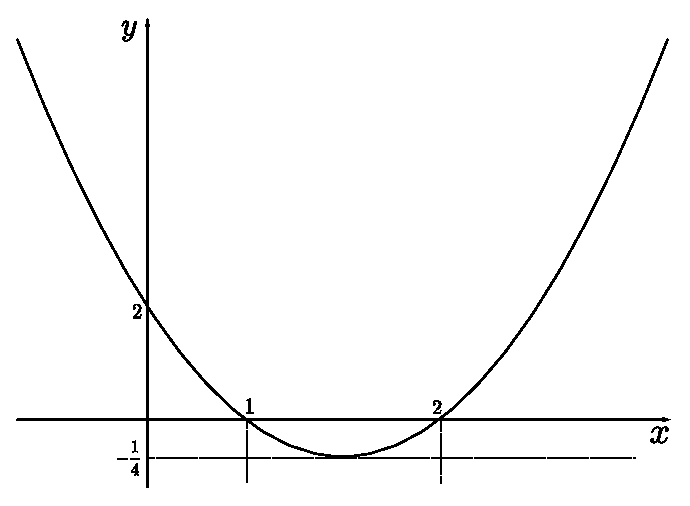
\includegraphics[scale=0.65]{img/quadratic-ex-1-6}
\captionstyle{\centering\it}
\caption{Quadratic graph given by $y=x^2-3x+2$.}
\label{fig:quadratic-ex-1-6}
\end{figure}

We know (from above):
\begin{itemize}
\item[(i)] the graph is a ``cup" rather than a ``cap" since the coefficient of $x^2$ is positive. Also we can easily see $P(0)=2$;
\item[(ii)] $P(x)=0$ at $x=1$ and $x=2$;
\item[(iii)] $P(x)$ is minimal at $x=\frac{3}{2}$ and $P\left(\frac{3}{2}\right)=-\frac{1}{4}$. Note, 
\[\left(x-\frac{3}{2}\right)^2-\frac{1}{4} \ge -\frac{1}{4},\] 
since anything squared is always positive!
\end{itemize}

